\section{Empirical Characterization of Constructive and Destructive Regimes}
\label{sec:gd-experiments}\label{sec:gd}

\begin{figure*}[!t]
\centering
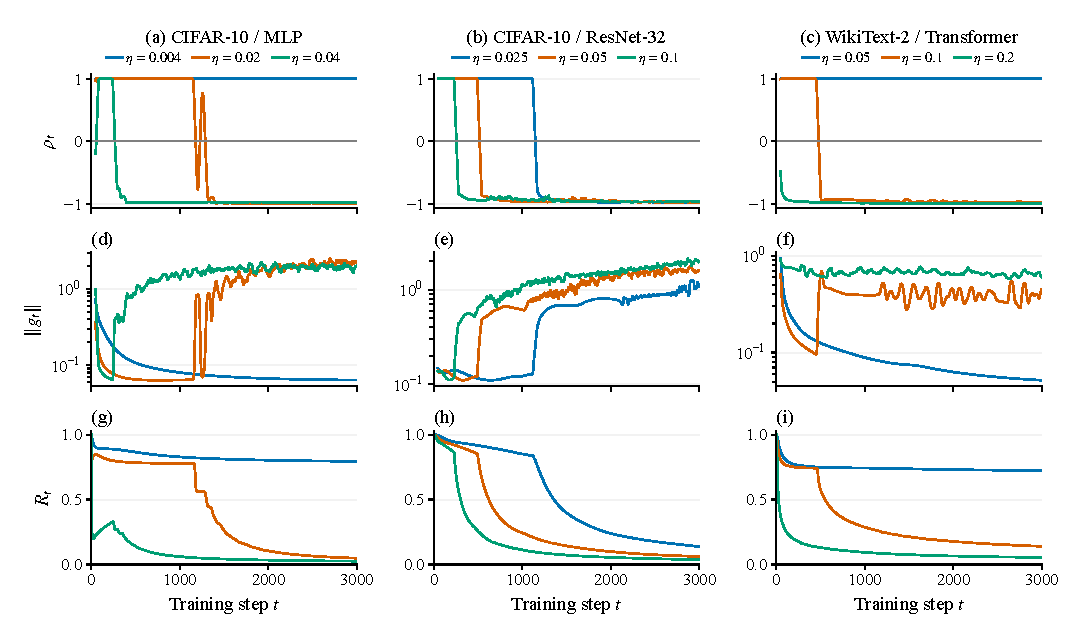
\includegraphics[width=\textwidth]{figures/gd_reversal_norm_retention.pdf}
\caption{Gradient alignment, magnitude, and accumulated displacement under full-batch GD. Top: cosine between consecutive gradients $\rho_t$. Middle: gradient norm $\|g_t\|$. Bottom: normalized displacement $R_t$. Gradient cosine and norm are smoothed using a trailing 50-step moving average.}
\label{fig:gd-alignment-displacement}
\end{figure*}

\begin{figure*}[!t]
\centering
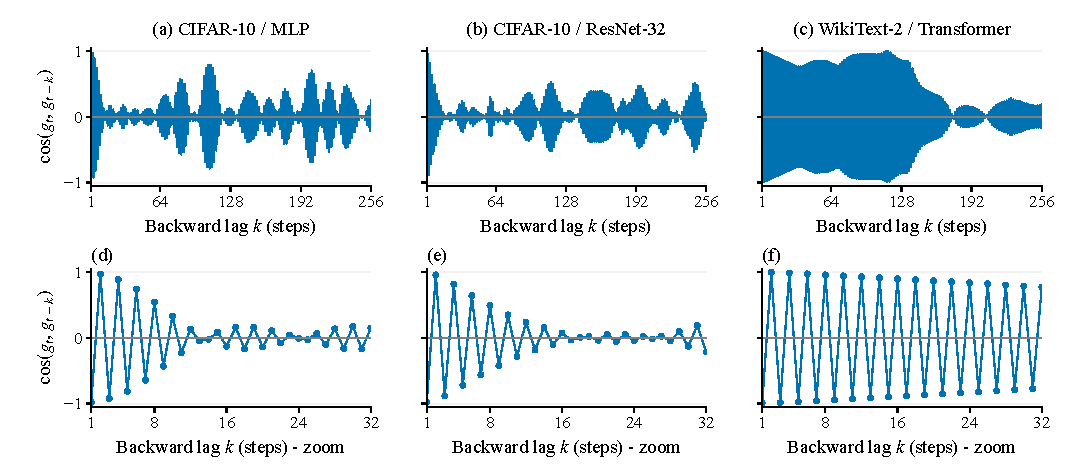
\includegraphics[width=\textwidth]{figures/gd_backward_compact.pdf}
\caption{Backward gradient alignment under full-batch GD at step $t=2256$, using the highest learning rate for each model. Each point shows $\cos(g_t,g_{t-k})$ at backward lag $k$. Top: lags 1--256; bottom: detail over lags 1--32.}
\label{fig:gd-backward}
\end{figure*}

\begin{figure*}[!t]
\centering
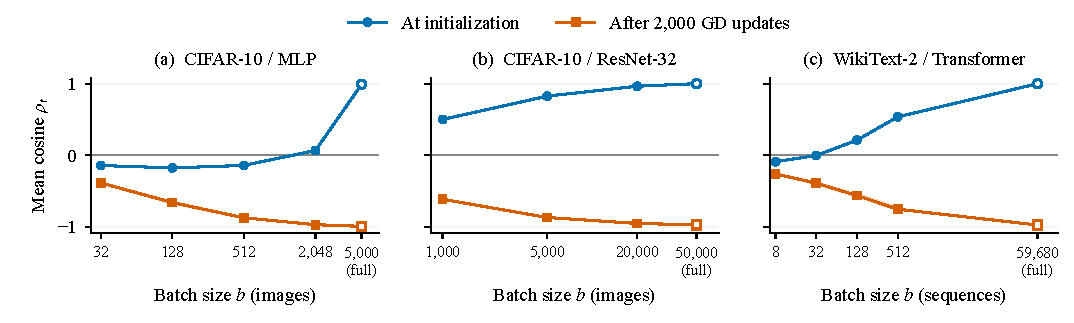
\includegraphics[width=\textwidth]{figures/sgd_batch_size_compact.pdf}
\caption{Mean gradient alignment $\rho_t$ across batch sizes during 200-update continuations from initialization (blue) and after 2,000 GD updates (orange). Lines show averages over eight sampling repetitions. Hollow markers denote full-batch GD. Learning rates are $0.02$ for the MLP and $0.1$ for ResNet and the Transformer. ResNet batches preserve BatchNorm groups, with a minimum size of 1,000 images.}
\label{fig:sgd-moving-geometry}
\end{figure*}

We empirically characterize the constructive and destructive regimes defined in Section~\ref{sec:regimes} using three settings from Cohen et al.~\cite{cohen2021edge}: a tanh MLP and a ResNet-32 trained on CIFAR-10, and a Transformer trained on WikiText-2. We first use full-batch GD to isolate learning dynamics from mini-batch sampling noise, comparing three learning rates from the same initialization over 3,000 updates for each model. We then vary batch size in separate runs initialized either from scratch or from a trained state to examine its effect on gradient alignment at different stages of training.

Figure~\ref{fig:gd-loss} shows oscillatory convergence across all three models. Oscillations emerge as scaled directional curvature $\eta\widehat{\kappa}_t$ approaches the threshold of $2$, where it remains even as scaled sharpness $\eta\lambda_{\max}$ increases further. At smaller learning rates, this transition is delayed or absent, while larger rates consistently lead to earlier oscillations. Figure~\ref{fig:gd-alignment-displacement} shows how this transition affects parameter updates. As $\eta\widehat\kappa_t$ approaches $2$, consecutive gradients become nearly opposite ($\rho_t\approx-1$), consistent with Eq.~\eqref{eq:kappa-estimate}. Gradient norms generally increase, but successive updates largely cancel one another, sharply reducing net parameter displacement relative to the distance traveled. At the highest learning rates, only 2.6\%, 3.7\%, and 5.4\% of the cumulative update magnitude remains as net displacement for the MLP, ResNet, and Transformer, respectively, after 3,000 updates. Despite the cancellation, these runs achieve the lowest final training loss for each model.

To examine how far gradient oscillations extend beyond consecutive updates, Fig.~\ref{fig:gd-backward} compares the current gradient with the preceding 256 gradients at the highest learning rate for each model. All three models exhibit strong alternating alignment at short lags, with nearly opposite gradients at odd lags and aligned gradients at even lags. This pattern weakens more rapidly in the MLP and ResNet than in the Transformer, but can reemerge at much longer lags. These results reveal persistent, structured oscillations rather than isolated reversals between consecutive updates.

From an optimization perspective, negative alignment is consistent with updates overshooting a local minimum along their direction and subsequently reversing. Unlike convergent oscillations on a fixed positive-definite quadratic, where gradient norms decrease, the destructive regime exhibits increasing gradient norms despite declining training loss. These repeated reversals lead to substantial cancellation of parameter updates, explaining the small net displacement observed in Figs.~\ref{fig:gd-alignment-displacement} and~\ref{fig:gd-backward}. From a representation-learning perspective, this raises the possibility that successive updates also interfere with previously learned structure.

\subsection{Mini-Batch Attenuation of Directional Alignment}
\label{sec:sgd-noise-experiments}

Equation~\eqref{eq:noise-cosine-approx} predicts that smaller batches bring expected gradient alignment closer to zero. We test this prediction over 200-update continuations from initialization and from states reached after 2,000 GD updates. Figure~\ref{fig:sgd-moving-geometry} shows that smaller batches weaken both positive alignment early in training and negative alignment in later trained states, consistently across all three models. This suggests that sampling noise may hinder constructive reinforcement while attenuating destructive oscillations, potentially contributing to its implicit regularization effects~\cite{haochen2021shape,smith2021origin}. Large-scale training often uses large batches~\cite{mccandlish2018largebatch,chowdhery2022palm}, which also reduces sampling variance. Whether that reduction amplifies instability during large-scale training remains open.
